\section{Topic Modelling}
\label{topic}
Topic Modelling is an unsupervised machine learning and statistical modelling approach which aims to discover the abstract `topics` in a collection of documents, referred to as the corpus. This can be used to find hidden semantic structures in a document. This works by looking at how often words appear in the corpus and trying to create topics made of words which are related to each other. For example an article about dogs would be more likely to have words such as `dog` and `bone`, and thus the topic model would most likely group those two words together into a topic. 

There are many approaches to topic modelling, one of the foremost examples is Latent Dirichlet Allocation \cite{blei2003latent}, which aims to reverse-engineer the topics by assuming the text was created from K topics and all words directly relate to one of the K topics. There are other forms of clustering algorithm which can be applied to words, such as the K Means clustering algorithm. 

\subsection{Latent Dirichlet Allocation}
Latent Dirichlet Allocation (LDA) is an unsupervised learning model which aims to collate words into K topics. When performing LDA, the text to be analysed is split into a series of documents, each composed of a bag of words where the order of the words does not matter. Most of the time, this will require pre-processing to remove words which do not contribute to the topics present in the work such as `the`, `is`,  and `a`. 

\noindent This algorithm assumes that the documents was made by first picking K topics, and any words present in the document belong to one of those K topics. The algorithm aims to reverse-engineer this process.
% START HERE 

Initially if the corpus is composed of a set of documents, D, the algorithm would first perform tokenisation so that each individual word is treated as a unique identity. Then each of the tokens for each of the documents would be parsed to remove the stop words. At this point each document is a list of tokens representing words which are not stop words. From this a document term matrix is created. This matrix has the dimensions $m$ x $v$, where M is the number of documents present in the corpus. V is the number of unique words present across all of the documents, or the vocabulary. This document term matrix records the term frequency of all of the words in the vocabulary for all of the documents present.

\begin{figure}[H]
	\centering
	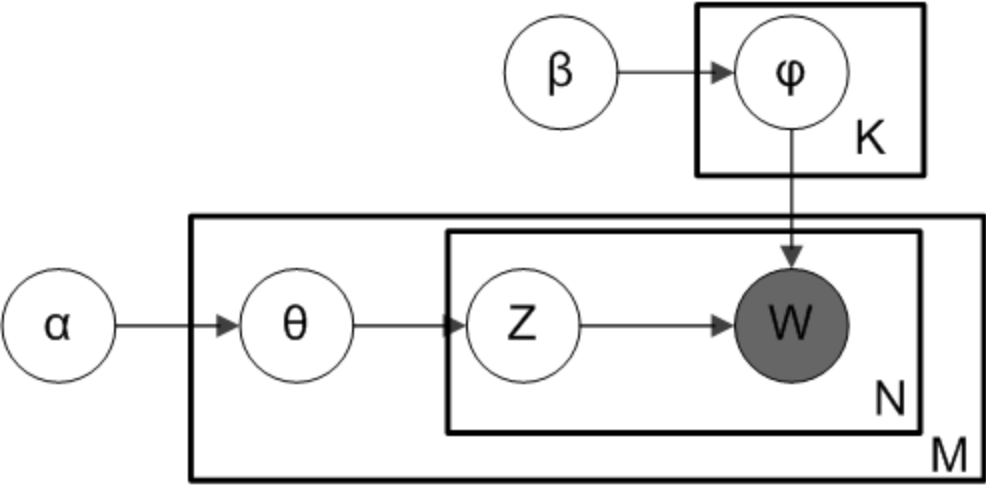
\includegraphics[width=0.6\textwidth]{images/LDA.png}
	\caption{A Graphical Plate representation of (smoothed) LDA (image from \cite{LDA})}
	\label{fig:ldafigure}
\end{figure}

The reverse-engineering process is shown graphically in Figure \ref{fig:ldafigure}. M denotes the number of documents, N refers to an individual document, and W refers to a single word, and is the only observable variable in the system. The algorithm assumes several matrices. \boldmath{$\varphi$} is defined as the word distribution across topics. In practice this is a matrix where \boldmath{$\varphi_{k}$} is the probability distribution across the V for topic K, such that \boldmath{$\varphi_{j, k}$} represents the probability that the \unboldmath{$j^{th}$} word in the vocabulary belongs in topic K. \boldmath{$\theta$} is defined as the topic distribution across documents, which means \boldmath{$\theta_{i}$} represents the topic distribution for document i, and that \boldmath{$\theta_{i, k}$} represents the probability of topic k being in document i. \textbf{}{Z} represents the matrix of documents and topics, where \textbf{$Z_{i,j}$} is the topic for the \unboldmath{$j^{th}$} word in document i. 

$\alpha$ and $\beta$ are the external parameters which control the initial distributions. $\alpha$ is the parameter which initially sets the shape of the topic distribution across documents, \boldmath{$\theta$}, and \unboldmath{$\beta$} is the parameter which initially sets the word distribution across topics, \boldmath{$\varphi$}. The aim is to optimise parameters \unboldmath{$\alpha$} and $\beta$ to find the best distribution of word and document probabilities which have generated the corpus most accurately. In the original paper \cite{blei2003latent}, both the topic-word distribution, $\beta$, and the topic-distributions, $\alpha$ can be modelled using a sparse Dirichlet prior, as it would be thought that the probability distribution of words in a topic and documents across topic would not necessarily be symmetric, and not all documents/words would contain all topics. Large values in $\alpha$ push the document topic distribution towards being more balanced between topics, and smaller alpha values push the document topic distribution probabilities towards being weighted more towards certain topics than being weighted evenly. 

The posterior probability is represented as below:
\begin{align*}
	p(\varphi_{1:k}, \theta_{1:M}, z_{1:M} | D; \alpha_{1:M}, \beta_{1:K})
\end{align*}

This can be calculated using variational inference, as the probability defined above is intractable. This entails calculating an approximation of the true posterior probability, and minimising the difference between the true posterior and the estimated posterior. In this case, the difference between the true and approximated posterior is the distance between them. To obtain the most accurate approximation, this distance has to be minimised which in this case is achieved by minimising the KL divergence between the approximation and the true posterior probability. The optimisation is shown below:
\begin{align*}
	\gamma^{*}, \phi^{*}, \lambda^{*} = argmin_{\gamma^{*}, \phi^{*}, \lambda^{*}} D(q(\varphi, \theta, z, | \gamma, \phi, \lambda) ||p(\varphi, \theta, z | D; \alpha, \beta))
\end{align*}


$\gamma$, $\phi$, and $\lambda$ are the free variational parameters used to approximate $\theta$, z, and $\varphi$ with. D(q||p) represents the KL divergence between q and p. Changing the $\gamma$, $\phi$, and $\lambda$ parameters changes the distance between the estimate, q, and the true posterior, p, and the aim is to find the values which minimises that distance.

In algorithmic terms this works on the basis of optimising one of $\varphi$, $\beta$, and \textbf{z} at a time. This is because these matrices are are intrinsically linked to one another. Pseudocode for the algorithm is shown below (Algorithm taken from \cite{ldaalgorithm}):
\begin{algorithm}
	\begin{algorithmic}
	\STATE Initialise Topics based on $\alpha$ and $\beta$\\
	repeat\\ 
	\hspace{1cm} for each document do\\
			\hspace{2cm} repeat\\ 
				\hspace{3cm}Update the topic assignment Variational parameters ($\theta$)\\
				\hspace{3cm}Update the topic proportions Variational parameters ($\varphi$)\\
			\hspace{2cm}until document objective converges\\
		\hspace{1cm}end for\\ 
		\hspace{1cm}update topics from aggregated per-document parameters (\textbf{z})\\
	until corpus objective converged\\
		\end{algorithmic}
\end{algorithm}

LDA has been used widely for topic modelling across many fields.  This has also been used in stock market predictions by attempting to mine many different kinds of data to used as prediction. This includes seeing if anything from social media data \cite{nguyen2015sentiment}, to topics in financial news \cite{feuerriegel2016analysis} affect stock prices. This is similar to the goal of this dissertation, and thus this was deemed a suitable metric to use for this purpose. 
 % END HERE
 \subsection{Term Frequency-Inverse Document Frequency}
 TF-IDF is a well known numeric statistic used to calculate the importance of a word to a document in a collection or corpus. It works based on of creating a weighting for each word, based on the product of the term frequency and the inverse document frequency. The term frequency is the count of how many times each word appeared in the document. The inverse document frequency aims to measure how much information a word provides to the document, i.e. if the word appears extremely often (e.g. the word `the`), it would attain a lower IDF score, and vice versa. It is calculated by taking the logarithm of the inverse of the fraction of documents which contain that word. The final TF-IDF value is calculated by multiplying the term frequency and inverse document frequencies together This is shown below:
 
 \begin{center}
 	$TF(t,d) = f_{t,d}$\\
 	$IDF(t, D) = log\frac{N}{\{d \in D : t \in D\}}$
 	$TF-IDF(t, d, D) = TF(t, d) * IDF(t, D) $
 \end{center}
 
The term frequency, \textit{tf}, for a term \textit{t}, in a document \textit{d}, is found by calculating the frequency of term \textit{t} in document \textit{d}. The inverse document frequency, for term \textit{t}, in a set of documents, \textit{D}, is the log of the number of documents in the corpus, \textit{N},  divided by the number of documents, \textit{d}, in the set of documents, where term \textit{t} is in the document.  
 
 TF-IDF is used extensively in text mining, as it shows the most important words of a corpus, this is used extensively, from paper recommender systems \cite{beel2016paper}, search engines \cite{xu2014pos}, and digital libraries \cite{philip2014application} alongside other uses. This has also been used extensively for predicting stock prices, as part of a wider prediction using sentiment analysis model. 
 
 
\subsection{K Means Clustering}
Another methodology of grouping objects together is to use a clustering technique such as the K Means algorithm. This algorithm, given a matrix X, of dimension \textit{n} x \textit{p}, where each row vector represents a point in p-dimensional space, places K candidate cluster centres randomly in p-dimensional space. Each of the points in p-dimensional space is allocated to the closest cluster. This is found for each point by calculating which cluster centre has the minimal distance to that point. 

The distance metric used for calculating distances between points in p-dimensional space can vary but it is most often the Euclidean Distance. The algorithm is an optimisation problem which aims to minimise the Within Cluster Sum of Squares, which is also the cluster variance. After assigning the points to the clusters, the location of the cluster centres are shifted to the mean of all of the points assigned to that cluster. Then the distances to the cluster centres are recalculated for all of the points, and the points are reassigned clusters to the cluster who's centre is the closest. This process of moving the cluster centres and reassigning the points continues until the assignments of the points to the clusters do not change. It should be noted that this algorithm is heavily dependant on the starting positions of the cluster centres, and is not guaranteed to find the optimal solution. As such it remains a computationally NP hard problem \cite{vattani2009hardness}. 
 
The K Means clustering algorithm only works with numerical data in n dimensions as it needs to quantify the distance between points. Thus if K means were used to cluster words, the words would have to be transformed into a numeric representation. A naive solution would be to just use the ASCII values of the words. However to perform clustering effectively based on the meaning of the words and relevance to the text as a whole, the numerical value would preserve any underlying relationship between the words and the document overall, which is not possible if ASCII was the one which was used. TF-IDF would be such a method, as it weights the importance of a word to a text, and the frequency of usage. 

This combined method of using TF-IDF with K Means is widely used. It has been used for summarisation of document spaces \cite{khan2019extractive}, for classification \cite{buana2012combination}, and specifically for topic detection \cite{6066301}. Thus, this was considered a suitable approach for topic classification.

\subsection{Mahalanobis distance}

Using the Euclidean distance for word clusters often presents a challenge, as the clusters may not end up being spherical in nature \cite{raykov2016k}, thus a different metric can be used, the Mahalanobis distance. This can also be used to calculate the distance between 2 points. This is calculated by measuring the number of standard deviations between points a and b, and can generalise to higher dimensions via the variance/covariance matrix.

The Mahalanobis distance would mainly be used after the cluster has been fitted (since the final variance covariance matrix is required), to calculate the distance between a point and the centres of the clusters. The Mahalanobis distance calculation is shown below. \textbf{X} is a matrix of $n$ vectors, such that \boldmath$x_{i}$ is a vector which represents a point in p-dimensional space. \boldmath$X_{c}$ represents the matrix where the points have been centred, and thus the variance covariance matrix can be calculated by matrix multiplying the transpose of the centred matrix and the centred matrix and dividing by the n -1, where n is the number of points. $\bar{ x  }$ refers to a vector, in this case a centroid, which represents a point in p-dimensional space. Thus the Mahalanobis distance is the square root of the difference between the point $x_{i}$ and the cluster centre$\bar{ x  }$, multiplied by the inverse of the variance covariance matrix, multiplied by the transpose of the difference between $x_{i}$ and the cluster centre. 


\begin{center}
	Covariance Matrix:
	\boldmath$C_{x} = \frac{1}{n - 1} (X_{c}) ^T (X_{c})$
	
	Mahalanobis Distance:
	\unboldmath$MD_{i}$ = \boldmath$\sqrt{(x_{i}  -  \bar{ x  } ) C_{x}^{-1} ( x_{i}   - \bar{ x  }  )^T    }  $
\end{center}

The Mahalanobis distance has been used with clustering algorithms such as k-means \cite{melnykov2014k} \cite{cerioli2005k}, and is frequently used in distributions of clusters which are either elliptical \cite{mitchell1985mahalanobis} or non normal distributions \cite{warren2011use}. Since the distribution of points around the k means clusters is likely to be unknown if TF-IDF is used to numerically transform the words, this was seen as a suitable metric to use for evaluating the clusters the algorithm would create.